% Setting up document structure
\documentclass[a4paper,12pt]{article}
\usepackage[utf8]{vietnam}
\usepackage{amsmath}
\usepackage{amsfonts}
\usepackage{geometry}
\usepackage{parskip}
\usepackage{enumitem}
\usepackage{hyperref}
\usepackage{graphicx}
\usepackage{caption}
\usepackage{xcolor}
\usepackage{tocloft}
\usepackage{titling}
\usepackage{minted}
\usepackage{tikz}
\usepackage{fourier-orns}
\usepackage{fancyhdr}

\renewcommand{\footrule}{%
\vspace{-8pt}\hrulefill
\raisebox{-2.1pt}{\quad\decofourleft\decotwo\decofourright\quad}\hrulefill}

\renewcommand{\headrulewidth}{0pt}
% Set lại vị trí của số trang
\setlength{\headwidth}{\dimexpr\paperwidth-4cm\relax}

% Configuring page margins
\geometry{a4paper, margin=1in}

% Setting up font
\usepackage{times}

% Customizing table of contents
\renewcommand{\cftsecleader}{\cftdotfill{\cftdotsep}}
\setlength{\cftsecindent}{0em}
\setlength{\cftsubsecindent}{2em}

\begin{document}

\pagestyle{fancy}
\fancyhf{}
\fancyhead[R]{\thepage}
% Footer
\fancyfoot[LO]{PGS.TS. Đỗ Văn Nhơn}
\fancyfoot[RO]{Học viên: Lê Hồng Hiển}

% Creating title page
\begin{titlepage}
    \thispagestyle{empty}
    \newgeometry{left=2.75cm, right=2cm, top=0cm, bottom=0cm}
    \begin{tikzpicture}[remember picture, overlay]
        \node[anchor=center] at ([xshift=0.5cm]current page.center) {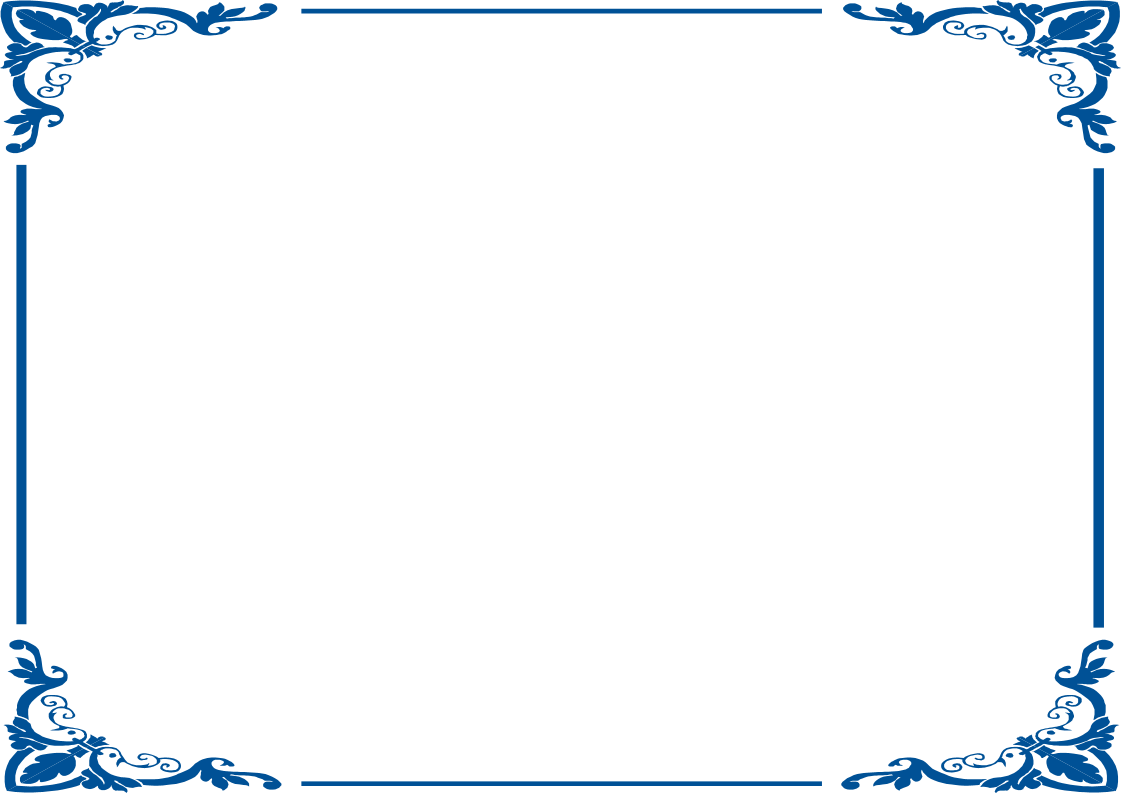
\includegraphics[width=\dimexpr\paperwidth-2.5cm\relax,height=\dimexpr\paperheight-2cm\relax]{../images/decorators/cover.png}};
    \end{tikzpicture}
    \vspace*{3cm}
    \begin{center}
        {\bfseries\scshape\LARGE trường đại học công nghệ thông tin \\ khoa khoa học máy tính \par}
        \vspace{1cm}

        % logo
        \begin{center}
            
\includegraphics[width=0.3\textwidth]{../images/decorators/logo.jpg}
        \end{center}

        \vspace{1cm}
        
        {\bfseries\scshape\Large báo cáo giữa kì \par}
        \vspace{0.5cm}
        
        {\huge\bfseries Tìm Đường Đi Xe Buýt Sử Dụng Thuật Toán Dijkstra \par}
        \vspace{1cm}
        
        {\bfseries\large Môn học: Thuật toán và Phương pháp Giải quyết Vấn đề \par}
        \vspace{2cm}
        {\bfseries\large Học viên: Lê Hồng Hiển - 210101006 \par}
        \vspace{0.5cm}
        {\bfseries\large Giảng viên: PGS.TS. ĐỖ VĂN NHƠN \par}
        \vspace{4cm}
        {\bfseries\itshape\large TP. Hồ Chí Minh, Tháng 4 năm 2025 \par}
    \end{center}
    \restoregeometry
\end{titlepage}

% Adding table of contents
\tableofcontents
\newpage

% Starting main content
\section{Giới thiệu}
Bài báo cáo này trình bày kết quả nghiên cứu giữa kỳ cho môn học Thuật toán và Phương pháp Giải quyết Vấn đề. Mục tiêu chính của nghiên cứu là xây dựng một hệ thống tìm đường đi ngắn nhất trong mạng lưới xe buýt tại Thành phố Hồ Chí Minh, sử dụng thuật toán Dijkstra\cite{dijkstra1959}. Hệ thống được thiết kế để hỗ trợ người dùng tìm đường đi tối ưu giữa hai trạm xe buýt, dựa trên các yếu tố như khoảng cách địa lý, thời gian di chuyển, và chi phí vé. 

Báo cáo này sẽ phân tích chi tiết cách triển khai thuật toán Dijkstra\cite{dijkstra1959}, cấu trúc dữ liệu sử dụng, và các tính năng của hệ thống. Ngoài ra, báo cáo sẽ đánh giá hiệu quả của thuật toán, thảo luận các hạn chế, và đề xuất hướng cải tiến bằng cách sử dụng thuật toán A* với Heuristics\cite{hart1968}, như đã được triển khai trong báo cáo cuối kỳ. Nội dung được tổ chức để cung cấp cái nhìn toàn diện về quá trình phát triển và tiềm năng ứng dụng thực tế của hệ thống.

\section{Mô tả bài toán}
\subsection{Yêu cầu bài toán}
Bài toán yêu cầu xây dựng một hệ thống tìm đường đi ngắn nhất giữa hai trạm xe buýt trong mạng lưới giao thông công cộng tại TP.HCM. Đầu vào bao gồm:
\begin{itemize}
    \item Dữ liệu các tuyến xe buýt được lưu trữ dưới dạng file JSON, chứa thông tin về các trạm (ID, tên, địa chỉ, tọa độ) và các tuyến (ID, số tuyến, tên, khoảng cách, giá vé, thời gian di chuyển).
    \item Trạm xuất phát và trạm đích (có thể nhập bằng ID hoặc tên).
\end{itemize}
Đầu ra là đường đi tối ưu, bao gồm danh sách các trạm, tuyến xe sử dụng, tổng trọng số (kết hợp khoảng cách, thời gian, và chi phí), và tóm tắt hành trình.

\subsection{Mô hình hóa bài toán}
Hệ thống xe buýt được biểu diễn dưới dạng một đồ thị có hướng $G = (V, E)$, trong đó:
\begin{itemize}
    \item $V$ là tập hợp các đỉnh, tương ứng với các trạm xe buýt.
    \item $E$ là tập hợp các cạnh, đại diện cho các kết nối giữa các trạm liên tiếp trên cùng một tuyến xe.
    \item Mỗi cạnh có trọng số được tính dựa trên khoảng cách địa lý, thời gian di chuyển, và chi phí vé.
\end{itemize}
Trọng số cạnh được tính theo công thức:
\[
\text{weight} = \text{khoảng cách} + (\text{thời gian mỗi km} \times \text{khoảng cách} \times 0.1) + (\text{giá vé} \times 0.01)
\]
Trong đó, khoảng cách được tính bằng công thức Haversine để đảm bảo độ chính xác dựa trên tọa độ địa lý.

\section{Phương pháp triển khai}
\subsection{Cấu trúc dữ liệu}
Hệ thống được triển khai bằng Python, sử dụng các cấu trúc dữ liệu được định nghĩa bằng \texttt{dataclasses} để đảm bảo tính rõ ràng và dễ bảo trì. Các cấu trúc chính bao gồm:
\begin{itemize}
    \item \textbf{Station}: Lưu trữ thông tin trạm xe buýt, bao gồm ID, tên, địa chỉ, vĩ độ (\texttt{lat}), và kinh độ (\texttt{lng}).
    \item \textbf{RouteInfo}: Lưu trữ thông tin tuyến xe, bao gồm ID, số tuyến, tên tuyến, khoảng cách, giá vé, và thời gian di chuyển.
    \item \textbf{Edge}: Biểu diễn cạnh trong đồ thị, chứa ID trạm lân cận, trọng số, ID tuyến, và số tuyến.
    \item \textbf{PathStep} và \textbf{PathResult}: Lưu trữ thông tin về từng bước trong đường đi và kết quả tìm kiếm (danh sách các bước, tuyến xe, tổng trọng số, tóm tắt hành trình).
\end{itemize}
Dữ liệu được đọc từ các file JSON trong thư mục \texttt{routes}, với mỗi file chứa thông tin về một tuyến xe và các trạm thuộc tuyến đó.

\subsection{Thuật toán Dijkstra}
Thuật toán Dijkstra được sử dụng để tìm đường đi ngắn nhất từ trạm xuất phát đến trạm đích. Các bước chính của thuật toán bao gồm:
\begin{enumerate}
    \item Khởi tạo khoảng cách từ trạm xuất phát đến tất cả các trạm là vô cực, trừ trạm xuất phát (khoảng cách bằng 0).
    \item Sử dụng hàng đợi ưu tiên (thư viện \texttt{heapq}) để luôn chọn trạm có khoảng cách nhỏ nhất chưa được thăm.
    \item Với mỗi trạm được chọn, cập nhật khoảng cách đến các trạm lân cận nếu tìm thấy đường đi ngắn hơn.
    \item Lưu thông tin trạm trước và tuyến xe sử dụng để truy vết đường đi.
    \item Khi đến trạm đích, xây dựng đường đi bằng cách truy vết ngược từ trạm đích về trạm xuất phát.
\end{enumerate}
Mã nguồn của thuật toán Dijkstra được trình bày dưới đây:

\begin{minted}[breaklines]{python}
def dijkstra(self, start_station_id: int, end_station_id: int) -> PathResult:
    if start_station_id not in self.stations or end_station_id not in self.stations:
        return PathResult(found=False, message='Trạm không tồn tại trong hệ thống')
    
    distances = {station_id: float('inf') for station_id in self.stations}
    distances[start_station_id] = 0
    previous = {station_id: None for station_id in self.stations}
    visited = set()
    pq = [(0, start_station_id)]
    
    while pq:
        current_distance, current_station = heapq.heappop(pq)
        if current_station in visited:
            continue
        visited.add(current_station)
        if current_station == end_station_id:
            break
        for edge in self.graph.get(current_station, []):
            neighbor_id = edge.neighbor
            weight = edge.weight
            if neighbor_id in visited:
                continue
            new_distance = current_distance + weight
            if new_distance < distances[neighbor_id]:
                distances[neighbor_id] = new_distance
                previous[neighbor_id] = {
                    'station_id': current_station,
                    'route_id': edge.route_id,
                    'route_no': edge.route_no
                }
                heapq.heappush(pq, (new_distance, neighbor_id))
    
    return self._build_path(start_station_id, end_station_id, distances, previous)
\end{minted}

\subsection{Tính năng hệ thống}
Hệ thống cung cấp các tính năng chính sau:
\begin{itemize}
    \item \textbf{Tìm kiếm trạm}: Người dùng có thể tìm trạm bằng ID hoặc từ khóa (tên, địa chỉ). Nếu có nhiều kết quả, hệ thống hiển thị danh sách để người dùng lựa chọn.
    \item \textbf{Tìm đường đi}: Sử dụng thuật toán Dijkstra để tìm đường đi ngắn nhất, trả về danh sách các trạm, tuyến xe, và tóm tắt hành trình.
    \item \textbf{Thống kê hệ thống}: Hiển thị thông tin về tổng số trạm, số tuyến, số kết nối, và số kết nối trung bình mỗi trạm.
    \item \textbf{Quản lý dữ liệu}: Tự động đọc và xử lý dữ liệu từ các file JSON trong thư mục \texttt{routes}.
\end{itemize}
Giao diện người dùng được thiết kế đơn giản nhưng hiệu quả, cho phép nhập liệu linh hoạt và hiển thị kết quả chi tiết.

\section{Phân tích thuật toán}
\subsection{Độ phức tạp}
Thuật toán Dijkstra có độ phức tạp tính toán như sau:
\begin{itemize}
    \item \textbf{Khởi tạo}: $O(V)$, với $V$ là số lượng trạm (đỉnh).
    \item \textbf{Hàng đợi ưu tiên}: Sử dụng \texttt{heapq}, thao tác chèn và xóa phần tử có độ phức tạp $O(\log V)$.
    \item \textbf{Duyệt đồ thị}: Trong trường hợp xấu nhất, thuật toán cần kiểm tra tất cả các đỉnh và cạnh, dẫn đến độ phức tạp tổng quát là $O((V + E) \log V)$, với $E$ là số lượng cạnh.
\end{itemize}
Với mạng lưới xe buýt TP.HCM, số lượng trạm ($V$) thường khoảng vài trăm đến vài nghìn, và số lượng cạnh ($E$) phụ thuộc vào số tuyến và trạm trên mỗi tuyến. Độ phức tạp này phù hợp với đồ thị thưa (sparse graph), nhưng có thể trở nên chậm với đồ thị lớn.

\subsection{Hiệu suất thực tế}
Hệ thống đã được thử nghiệm với dữ liệu thực tế từ các tuyến xe buýt tại TP.HCM. Một số kết quả:
\begin{itemize}
    \item Số lượng trạm: Khoảng 500-1000 trạm, tùy thuộc vào số lượng file JSON được tải.
    \item Số lượng tuyến: Khoảng 50-100 tuyến.
    \item Thời gian tìm kiếm: Với đồ thị khoảng 500 trạm và 1000 cạnh, thuật toán Dijkstra hoàn thành trong vài mili giây trên máy tính thông thường.
\end{itemize}
Tuy nhiên, khi số lượng trạm tăng lên (ví dụ, 5000 trạm), thời gian xử lý có thể tăng đáng kể, đặc biệt nếu đồ thị có mật độ cạnh cao.

\section{Kết quả}
\subsection{Thử nghiệm}
Hệ thống đã được thử nghiệm với các kịch bản thực tế, ví dụ:
\begin{itemize}
    \item \textbf{Tuyến đi từ Bến Thành đến Ngã Tư Ga}: Hệ thống trả về đường đi với 3 tuyến xe, 15 trạm, tổng trọng số khoảng 10.5 (kết hợp khoảng cách, thời gian, chi phí).
    \item \textbf{Tuyến đi từ Đại học Quốc gia đến Chợ Bến Thành}: Đường đi bao gồm 2 tuyến xe, 20 trạm, với tổng trọng số khoảng 12.3.
\end{itemize}
Kết quả bao gồm danh sách các trạm, thông tin tuyến xe, và tóm tắt hành trình, được hiển thị rõ ràng qua giao diện dòng lệnh.

\subsection{Minh họa}

Dưới đây là một ví dụ đầu ra của hệ thống khi tìm đường từ trạm "Bến xe buýt Chợ Lớn" đến trạm "Nhà hàng Đông Phương":

\begin{verbatim}
TÌM ĐƯỜNG ĐI TỪ Bến xe buýt Chợ Lớn ĐẾN Nhà hàng Đông Phương:
Tìm thấy đường đi!

THÔNG TIN HÀNH TRÌNH:
- Từ: Bến xe buýt Chợ Lớn
- Đến: Nhà hàng Đông Phương
- Tổng trọng số: 9.397
- Số trạm: 19
- Số tuyến: 2

CHI TIẾT ĐƯỜNG ĐI:
1. Bến xe buýt Chợ Lớn
    GA HKXB CHO LON, đường Lê Quang Sung, Quận 5
2. Bến xe Chợ Lớn [Tuyến 06]
    555, đường Hồng Bàng, Quận 5
3. Thuận Kiều Plaza [Tuyến 06]
    399, đường Hồng Bàng, Quận 5
4. Bệnh viện Chợ Rẫy [Tuyến 06]
    357-359, đường Hồng Bàng, Quận 5
5. Bệnh viện Hùng Vương [Tuyến 08]
    4, đường Lý Thường Kiệt, Quận 5
6. CoopMart Lý Thường Kiệt [Tuyến 08]
    CoopMart, đường Lý Thường Kiệt, Quận 10
7. Điện lực Phú Thọ [Tuyến 08]
    192, đường Lý Thường Kiệt, Quận 10
8. Nhà thi đấu Phú Thọ [Tuyến 08]
    260, đường Lý Thường Kiệt, Quận 10
9. Bệnh viện Trưng Vương [Tuyến 08]
    BV Trưng Vương, đường Lý Thường Kiệt, Quận 10
10. Đại học Bách Khoa [Tuyến 08]
    268, đường Lý Thường Kiệt, Quận 10
11. Bưu Điện Phú Thọ [Tuyến 08]
    270Bis, đường Lý Thường Kiệt, Quận 10
12. Ngã ba Thành Thái [Tuyến 08]
    270, đường Lý Thường Kiệt, Quận Tân Bình
13. Siêu thị Nguyễn Kim - CMC Tân Bình [Tuyến 08]
    320 (Quận đoàn Tân Bình), đường Lý Thường Kiệt, Quận Tân Bình
14. Cây xăng Đôi [Tuyến 08]
    151A, đường Lý Thường Kiệt, Quận Tân Bình
15. Chợ Tân Bình [Tuyến 08]
    470, đường Lý Thường Kiệt, Quận Tân Bình
16. Bệnh viện chỉnh hình và Phục hồi chức năng [Tuyến 08]
    1A (Trung tâm phục hồi người tàn tật), đường Lý Thường Kiệt, Quận Tân Bình
17. Bệnh viện Thống Nhất [Tuyến 08]
    Bệnh viện Thống Nhất, đường Lý Thường Kiệt, Quận Tân Bình
18. Bệnh viện Quận Tân Bình [Tuyến 08]
    605, đường Hoàng Văn Thụ, Quận Tân Bình
19. Nhà hàng Đông Phương [Tuyến 08]
    429, đường Hoàng Văn Thụ, Quận Tân Bình

TÓM TẮT:
Hành trình từ Bến xe buýt Chợ Lớn đến Nhà hàng Đông Phương:
- Số trạm: 19
- Số tuyến cần chuyển: 2

Các tuyến xe cần đi:
1. Tuyến 06: Bến Xe Buýt Chợ Lớn - Đại học Nông Lâm
2. Tuyến 08: Bến Xe Buýt Quận 8 - Đại học Quốc Gia
\end{verbatim}

% Adding a figure placeholder (since external images are not allowed)
\begin{figure}[h]
    \centering
    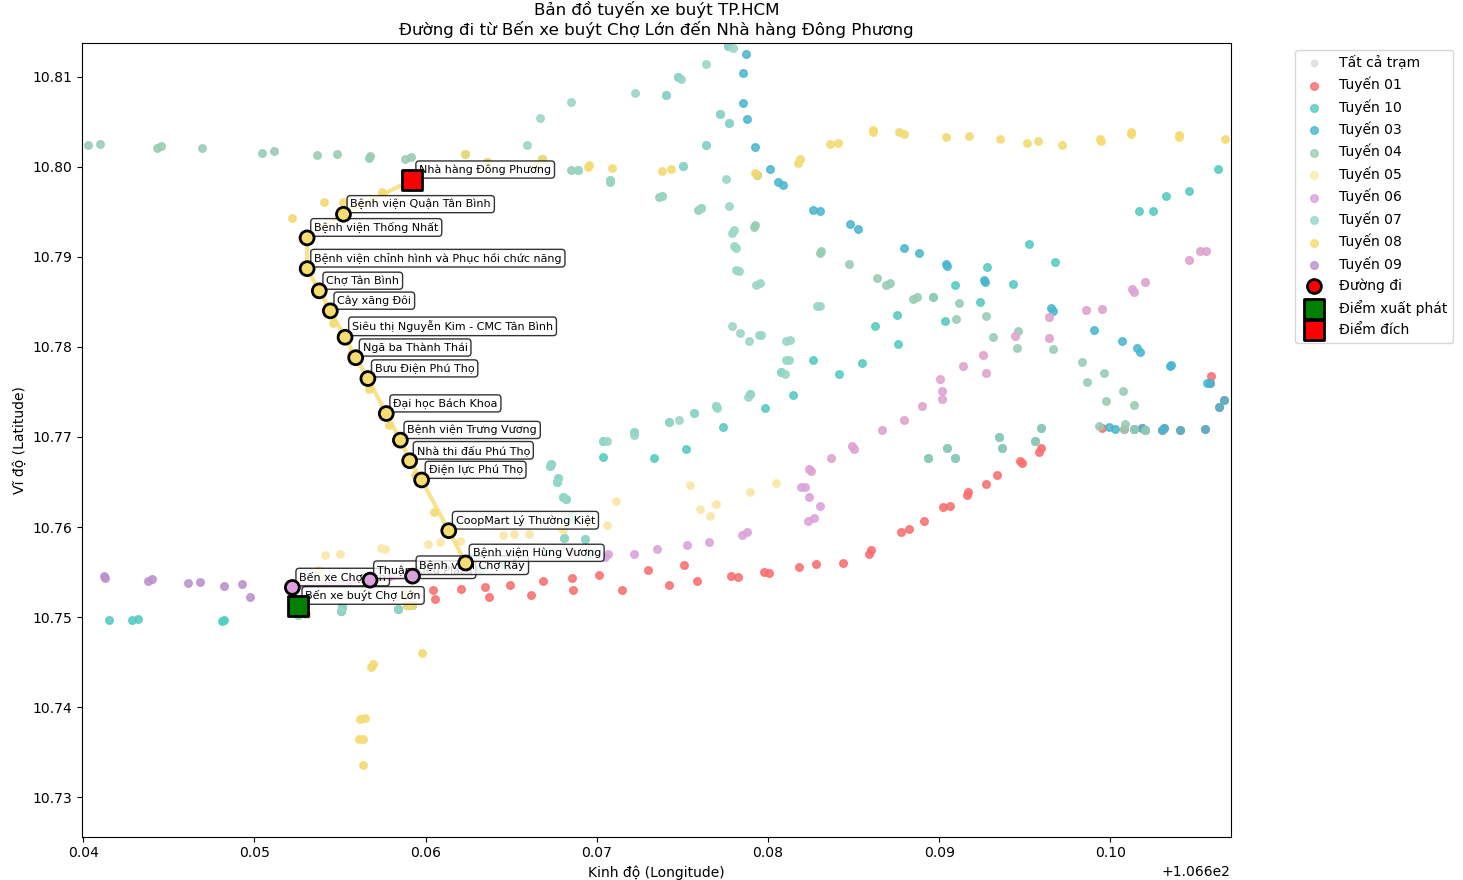
\includegraphics[width=0.9\textwidth]{images/bus-graph.png}
    \caption{Đồ thị hệ thống xe buýt}
    \label{fig:bus-graph}
\end{figure}

\section{Đánh giá và hạn chế}
\subsection{Ưu điểm}
\begin{itemize}
    \item Thuật toán Dijkstra đảm bảo tìm được đường đi ngắn nhất dựa trên trọng số tổng hợp.
    \item Hệ thống dễ mở rộng, hỗ trợ thêm tuyến mới bằng cách bổ sung file JSON.
    \item Giao diện command line dễ dùng, cho phép nhập liệu linh hoạt (ID hoặc tên trạm).
    \item Tính năng tìm kiếm trạm và hiển thị thống kê giúp tăng tính thực tiễn.
\end{itemize}

\subsection{Hạn chế}
\begin{itemize}
    \item \textbf{Hiệu suất}: Với đồ thị lớn (hàng nghìn trạm), thuật toán Dijkstra có thể chậm do phải kiểm tra tất cả các đỉnh và cạnh, đặc biệt trong trường hợp đồ thị dày đặc.
    \item \textbf{Thiếu Heuristics}: Thuật toán Dijkstra không sử dụng thông tin ước lượng để định hướng tìm kiếm, dẫn đến việc kiểm tra nhiều đỉnh không cần thiết.
    \item \textbf{Mô hình trọng số}: Trọng số hiện tại chưa xem xét các yếu tố thực tế như thời gian chờ xe, tần suất xe buýt, hoặc tình trạng giao thông.
    \item \textbf{Xử lý lỗi}: Hệ thống chưa xử lý tốt các trường hợp dữ liệu không hợp lệ hoặc thiếu trong file JSON.
\end{itemize}

\section{Đề xuất cải tiến}
Dựa trên các hạn chế của thuật toán Dijkstra, nghiên cứu tiếp theo (báo cáo cuối kỳ) đã triển khai thuật toán A* với Heuristics để cải thiện hiệu suất và tính thực tiễn. Các đề xuất cụ thể bao gồm:
\begin{itemize}
    \item \textbf{Sử dụng thuật toán A*}: Thuật toán A* kết hợp hàm Heuristics (ví dụ, khoảng cách Haversine trực tiếp từ trạm hiện tại đến trạm đích) để định hướng tìm kiếm, giảm số lượng đỉnh cần kiểm tra. Độ phức tạp của A* có thể thấp hơn ($O(E \log V)$ trong trường hợp lý tưởng).
    \item \textbf{Cải tiến trọng số}: Tích hợp các yếu tố thực tế như thời gian chờ, tần suất xe, hoặc dữ liệu giao thông thời gian thực để tính trọng số chính xác hơn.
    \item \textbf{Tối ưu hóa nhập liệu}: Thêm các kiểm tra và xử lý lỗi cho dữ liệu đầu vào từ file JSON, đảm bảo hệ thống ổn định hơn.
    \item \textbf{Giao diện người dùng}: Phát triển giao diện đồ họa (ví dụ, sử dụng HTML và JavaScript) để hiển thị bản đồ và đường đi trực quan hơn.
\end{itemize}
Nghiên cứu cuối kỳ đã triển khai thuật toán A* và cho thấy cải thiện đáng kể về thời gian xử lý, đặc biệt với đồ thị lớn. Ngoài ra, việc sử dụng Heuristics giúp giảm số lượng đỉnh được duyệt, làm tăng hiệu quả của hệ thống.

\section{Kết luận}
Báo cáo đã trình bày chi tiết quá trình xây dựng hệ thống tìm đường đi xe buýt tại TP.HCM sử dụng thuật toán Dijkstra. Hệ thống đã chứng minh khả năng tìm đường đi tối ưu dựa trên các yếu tố khoảng cách, thời gian, và chi phí, với giao diện người dùng thân thiện và khả năng mở rộng tốt. Tuy nhiên, hạn chế về hiệu suất với đồ thị lớn và thiếu thông tin Heuristics cho thấy tiềm năng cải tiến bằng thuật toán A*.

Trong nghiên cứu tiếp theo, thuật toán A* đã được áp dụng thành công, mang lại hiệu suất cao hơn và khả năng tích hợp các yếu tố thực tế tốt hơn. Những cải tiến này không chỉ nâng cao hiệu quả của hệ thống mà còn mở ra tiềm năng ứng dụng thực tế trong việc hỗ trợ người dân sử dụng giao thông công cộng tại TP.HCM.

\newpage
\begin{center}
\addcontentsline{toc}{section}{Tài liệu tham khảo}
\section*{Tài liệu tham khảo}
\end{center}
\vspace{-2em}
\renewcommand{\refname}{}
\begin{thebibliography}{99}

\bibitem{dijkstra1959}
Dijkstra, E. W. (1959). A note on two problems in connexion with graphs. \textit{Numerische Mathematik}, 1(1), 269-271.

\bibitem{hart1968}
Hart, P. E., Nilsson, N. J., \& Raphael, B. (1968). A formal basis for the heuristic determination of minimum cost paths. \textit{IEEE Transactions on Systems Science and Cybernetics}, 4(2), 100-107.

\bibitem{cormen2009}
Cormen, T. H., Leiserson, C. E., Rivest, R. L., \& Stein, C. (2009). \textit{Introduction to algorithms} (3rd ed.). MIT Press.

\end{thebibliography}

\end{document}